
\documentclass[conference]{IEEEtran}
% Some Computer Society conferences also require the compsoc mode option,
% but others use the standard conference format.
%
% If IEEEtran.cls has not been installed into the LaTeX system files,
% manually specify the path to it like:
% \documentclass[conference]{../sty/IEEEtran}





% Some very useful LaTeX packages include:
% (uncomment the ones you want to load)


% *** CITATION PACKAGES ***
%
%\usepackage{cite}
% cite.sty was written by Donald Arseneau
% V1.6 and later of IEEEtran pre-defines the format of the cite.sty package
% \cite{} output to follow that of the IEEE. Loading the cite package will
% result in citation numbers being automatically sorted and properly
% "compressed/ranged". e.g., [1], [9], [2], [7], [5], [6] without using
% cite.sty will become [1], [2], [5]--[7], [9] using cite.sty. cite.sty's
% \cite will automatically add leading space, if needed. Use cite.sty's
% noadjust option (cite.sty V3.8 and later) if you want to turn this off
% such as if a citation ever needs to be enclosed in parenthesis.
% cite.sty is already installed on most LaTeX systems. Be sure and use
% version 5.0 (2009-03-20) and later if using hyperref.sty.
% The latest version can be obtained at:
% http://www.ctan.org/pkg/cite
% The documentation is contained in the cite.sty file itself.






% *** GRAPHICS RELATED PACKAGES ***
%
\ifCLASSINFOpdf
  \usepackage[pdftex]{graphicx}
  % declare the path(s) where your graphic files are
  % \graphicspath{{../pdf/}{../jpeg/}}
  % and their extensions so you won't have to specify these with
  % every instance of \includegraphics
  % \DeclareGraphicsExtensions{.pdf,.jpeg,.png}
\else
  % or other class option (dvipsone, dvipdf, if not using dvips). graphicx
  % will default to the driver specified in the system graphics.cfg if no
  % driver is specified.
  % \usepackage[dvips]{graphicx}
  % declare the path(s) where your graphic files are
  % \graphicspath{{../eps/}}
  % and their extensions so you won't have to specify these with
  % every instance of \includegraphics
  % \DeclareGraphicsExtensions{.eps}
\fi


% *** MATH PACKAGES ***
%
\usepackage{amsmath}
% A popular package from the American Mathematical Society that provides
% many useful and powerful commands for dealing with mathematics.
%
% Note that the amsmath package sets \interdisplaylinepenalty to 10000
% thus preventing page breaks from occurring within multiline equations. Use:
%\interdisplaylinepenalty=2500
% after loading amsmath to restore such page breaks as IEEEtran.cls normally
% does. amsmath.sty is already installed on most LaTeX systems. The latest
% version and documentation can be obtained at:
% http://www.ctan.org/pkg/amsmath





% *** SPECIALIZED LIST PACKAGES ***
%
%\usepackage{algorithmic}
% algorithmic.sty was written by Peter Williams and Rogerio Brito.
% This package provides an algorithmic environment fo describing algorithms.
% You can use the algorithmic environment in-text or within a figure
% environment to provide for a floating algorithm. Do NOT use the algorithm
% floating environment provided by algorithm.sty (by the same authors) or
% algorithm2e.sty (by Christophe Fiorio) as the IEEE does not use dedicated
% algorithm float types and packages that provide these will not provide
% correct IEEE style captions. The latest version and documentation of
% algorithmic.sty can be obtained at:
% http://www.ctan.org/pkg/algorithms
% Also of interest may be the (relatively newer and more customizable)
% algorithmicx.sty package by Szasz Janos:
% http://www.ctan.org/pkg/algorithmicx




% *** ALIGNMENT PACKAGES ***
%
%\usepackage{array}
% Frank Mittelbach's and David Carlisle's array.sty patches and improves
% the standard LaTeX2e array and tabular environments to provide better
% appearance and additional user controls. As the default LaTeX2e table
% generation code is lacking to the point of almost being broken with
% respect to the quality of the end results, all users are strongly
% advised to use an enhanced (at the very least that provided by array.sty)
% set of table tools. array.sty is already installed on most systems. The
% latest version and documentation can be obtained at:
% http://www.ctan.org/pkg/array


% IEEEtran contains the IEEEeqnarray family of commands that can be used to
% generate multiline equations as well as matrices, tables, etc., of high
% quality.

% *** FLOAT PACKAGES ***
%
%\usepackage{fixltx2e}
% fixltx2e, the successor to the earlier fix2col.sty, was written by
% Frank Mittelbach and David Carlisle. This package corrects a few problems
% in the LaTeX2e kernel, the most notable of which is that in current
% LaTeX2e releases, the ordering of single and double column floats is not
% guaranteed to be preserved. Thus, an unpatched LaTeX2e can allow a
% single column figure to be placed prior to an earlier double column
% figure.
% Be aware that LaTeX2e kernels dated 2015 and later have fixltx2e.sty's
% corrections already built into the system in which case a warning will
% be issued if an attempt is made to load fixltx2e.sty as it is no longer
% needed.
% The latest version and documentation can be found at:
% http://www.ctan.org/pkg/fixltx2e


%\usepackage{stfloats}
% stfloats.sty was written by Sigitas Tolusis. This package gives LaTeX2e
% the ability to do double column floats at the bottom of the page as well
% as the top. (e.g., "\begin{figure*}[!b]" is not normally possible in
% LaTeX2e). It also provides a command:
%\fnbelowfloat
% to enable the placement of footnotes below bottom floats (the standard
% LaTeX2e kernel puts them above bottom floats). This is an invasive package
% which rewrites many portions of the LaTeX2e float routines. It may not work
% with other packages that modify the LaTeX2e float routines. The latest
% version and documentation can be obtained at:
% http://www.ctan.org/pkg/stfloats
% Do not use the stfloats baselinefloat ability as the IEEE does not allow
% \baselineskip to stretch. Authors submitting work to the IEEE should note
% that the IEEE rarely uses double column equations and that authors should try
% to avoid such use. Do not be tempted to use the cuted.sty or midfloat.sty
% packages (also by Sigitas Tolusis) as the IEEE does not format its papers in
% such ways.
% Do not attempt to use stfloats with fixltx2e as they are incompatible.
% Instead, use Morten Hogholm'a dblfloatfix which combines the features
% of both fixltx2e and stfloats:
%
% \usepackage{dblfloatfix}
% The latest version can be found at:
% http://www.ctan.org/pkg/dblfloatfix




% *** PDF, URL AND HYPERLINK PACKAGES ***
%
%\usepackage{url}
% url.sty was written by Donald Arseneau. It provides better support for
% handling and breaking URLs. url.sty is already installed on most LaTeX
% systems. The latest version and documentation can be obtained at:
% http://www.ctan.org/pkg/url
% Basically, \url{my_url_here}.




% *** Do not adjust lengths that control margins, column widths, etc. ***
% *** Do not use packages that alter fonts (such as pslatex).         ***
% There should be no need to do such things with IEEEtran.cls V1.6 and later.
% (Unless specifically asked to do so by the journal or conference you plan
% to submit to, of course. )


% correct bad hyphenation here
\hyphenation{op-tical net-works semi-conduc-tor}


\begin{document}
%
% paper title
% Titles are generally capitalized except for words such as a, an, and, as,
% at, but, by, for, in, nor, of, on, or, the, to and up, which are usually
% not capitalized unless they are the first or last word of the title.
% Linebreaks \\ can be used within to get better formatting as desired.
% Do not put math or special symbols in the title.
\title{Power Allocation and Relay Selection in
Amplify-and-Forward Relaying
}


% author names and affiliations
% use a multiple column layout for up to three different
% affiliations
\author{\IEEEauthorblockN{Prudhvi Porandla \quad Prof. Prasanna Chaporkar}
\IEEEauthorblockA{ Electrical Engineering\\
Indian Institute of Technology Bombay\\
}
}


% use for special paper notices
%\IEEEspecialpapernotice{(Invited Paper)}




% make the title area
\maketitle

% As a general rule, do not put math, special symbols or citations
% in the abstract
\begin{abstract}
	Multihop communication is considered to be a standard in next generation
	cellular networks.  There are several relaying schemes,
	Decode-and-forward(DF) and Amplify-and-Forward(AF) being the popular ones.
	In DF scheme, the relay decodes the message from the source, re-encodes
	and transmits it to the destination node whereas in AF the relay amplifies
	the received signal and transmits to the destination node. Relay selection
	and optimal power allocation are two important aspects in either
	scheme. In this work, we look at these two problems in 2-hop communication
	network in which relays employ AF scheme. However, when there are multiple
	relays the power allocation might interfere with relay selection. We show
	that this is indeed the case and discuss the conditions under which a relay
	switch over can take place.

\end{abstract}

% no keywords




% For peer review papers, you can put extra information on the cover page as
% needed: \ifCLASSOPTIONpeerreview \begin{center} \bfseries EDICS Category:
% 3-BBND \end{center} \fi
%
% For peerreview papers, this IEEEtran command inserts a page break and creates
% the second title. It will be ignored for other modes.
\IEEEpeerreviewmaketitle



\section{Introduction}
% no \IEEEPARstart
Cooperative communication is an efficient way to use network 
resources to increase rate and coverage in cellular networks.
Currently, network provider places the relay in an optimum
position so that the relay to base station link is always good. 
In next generation cellular networks, user-assisted relaying is being 
considered a standard. The idea is based on the fact that around
a transmitting user there will be many idle user equipments which can 
 be used as relays. That means the standard should allow users to 
send signals directly to nearby users without going through base station.
There are many challenges that need to be solved to be able to do
this correctly considering that virtually every user thinks this is 
risks their privacy. New incentive mechanisms need to be developed 
to compensate the relaying users for the extra power spent. Apart from
security and billing issues, there are also some engineering challenges
like optimising power at both relay and source nodes, selecting the best relay 
etc. \\ 
Two popular relaying schemes are Decode-and-Forward and Amplify-and-Forward.
In partial decode-and-forward scheme, the whole message is split in to a private
part and a public part. In the first slot, the source node broadcasts the public
part to relay node and destination node. The relay decodes the message and reencodes
it using an independent codebook and transmits to destination in the second slot.
The source transmits the private part in second slot. The destination node 
receives public part from source in the first slot and in second slot it
receives re-encoded public part from relay node and private part from source node.
This scheme imposes severe restrictions on timing and synchronization at 
different stages of transmission. This is one of the reasons why amplify-and-forward
scheme is considered more viable although rate gain is higher in DF scheme. \\
In previous works, many relay selection schemes have been proposed but most 
of them are not based on SNR. For such schemes source power does not affect 
relay selection. In an SNR based relay selection policy, source
power and relay power affects relay selection. 
 However, this may not always be the case; 
under some channel conditions power allocation does not affect relay selection.
In this work, we assume relay power is constant and provide an intuitive
understanding of the conditions
under which a relay switch over can take place and under what conditions
the relay selection problem and power allocation problem are independent.



%\begin{figure}[!t] \centering \includegraphics[width=2.5in]{myfigure} where an
%.eps filename suffix will be assumed under latex, and a .pdf suffix will be
%assumed for pdflatex; or what has been declared via
%\DeclareGraphicsExtensions.  \caption{Simulation results for the network.}
%\label{fig_sim} \end{figure}

%\begin{figure*}[!t] \centering \subfloat[Case
%I]{\includegraphics[width=2.5in]{box}% \label{fig_first_case}} \hfil
%\subfloat[Case II]{\includegraphics[width=2.5in]{box}%
%\label{fig_second_case}} \caption{Simulation results for the network.}
%\label{fig_sim} \end{figure*}
%
%\begin{table}[!t]
%% increase table row spacing, adjust to taste
%\renewcommand{\arraystretch}{1.3} if using array.sty, it might be a good idea
%to tweak the value of \extrarowheight as needed to properly center the text
%within the cells \caption{An Example of a Table} \label{table_example}
%\centering
%% Some packages, such as MDW tools, offer better commands for making tables
%% than the plain LaTeX2e tabular which is used here.
%\begin{tabular}{|c||c|} \hline One & Two\\ \hline Three & Four\\ \hline
%\end{tabular} \end{table}



\section{Amplify-and-Forward Relaying}
Consider 2-hop relaying; we have a source node, the destination, and a relay
node. In amplify-and-forward(AF) relaying scheme, the total transmission period is
divided in to two slots.
In the first slot, source node broadcasts the message to relay and destination nodes
and in the second the relay amplifies the received signal and retransmits it to 
the destination node. This is illustrated in fig~\ref{twoSlots}.
\begin{figure}[!t] 
	\centering 
	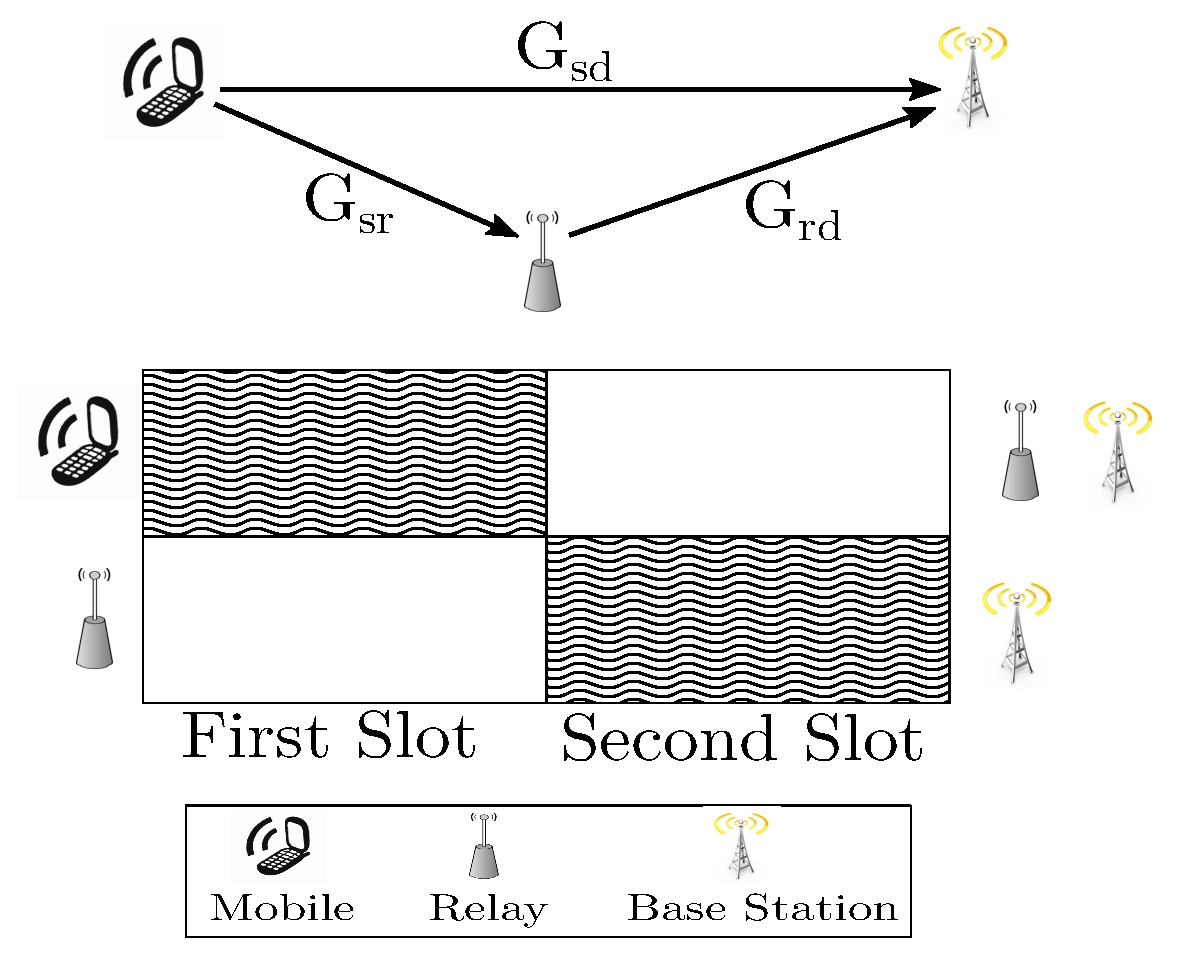
\includegraphics[width=2.5in]{img/sysmodel.eps} 
	\caption{Two slots in AF}
	\label{twoSlots} 
\end{figure}
\subsection{Received Signals }
The signals received at relay and destination nodes in the two slots are as 
follows:\\
\textit{First Slot:}
\begin{align} \label{ysd}
	Y_{sd} &= \sqrt{P_s G_{sd}} X_s + n_{sd}
\end{align}
\begin{align*}
	Y_{sr} &= \sqrt{P_s G_{sr}} X_s + n_{sr} \\
\end{align*}
\textit{Second Slot:}
\begin{equation}\label{yrd}
	Y_{rd} = \sqrt{P_r G_{rd}} X_{rd} + n_{rd} 
\end{equation}
\begin{equation} \label{finalyrd}
	Y_{rd} = \frac{\sqrt{\mathstrut P_r G_{rd} P_s G_{sr}}}{\sqrt{\mathstrut 
	P_s G_{sr} + \sigma^2}}X_s + \frac{\sqrt{\mathstrut P_rG_{rd}}}{\sqrt{\mathstrut 
	P_s G_{sr} + \sigma^2}} n_{sr} + n_{rd} 
\end{equation}
The final expression for $Y_{rd}$ is obtained by substituting
$X_{rd} = \frac{Y_{sr}}{|Y_{sr}|}$ in eq.~\ref{yrd}. All symbols have usual
meanings - $s$ denotes source, $P$ denotes power, $G_{sd}\big(=\dfrac{g_{sd}}
{d^2_{sd}}\big)$ is the channel gain from source to destination, etc.
\subsection{Rate}
The rate/capacity of AF relaying scheme is given by
\begin{align*}
	R = \frac{1}{2} w \log_2(1+\Gamma_{sd}+\Gamma_{rd}) 
	\\ \text{where $\Gamma$
represents SNR}
\end{align*}
Substituting $\Gamma_{sd}$ and $\Gamma_{rd}$, obtained from equations \ref{ysd}
and \ref{finalyrd} respectively, in the above expression we get
\begin{align*}
	R &= \frac{1}{2} w \log_2\bigg(1+\frac{P_s G_{sd}}{\sigma^2} +
	\frac{P_s G_{sr} P_r G_{rd}}{\sigma^2(\sigma^2 + P_sG_{sr} + P_rG_{rd})}\bigg)
\end{align*}

\section{Source power and Relay selection}
When there are multiple relays we have to select one of them for transmission. 
There are various relay selection techniques one of which is Max-Min selection-
relay $i$ which maximizes min\{$G_{sr_i},G_{r_id}$\} is selected -  and a 
continuous version of this scheme which uses harmonic mean of $G_{sr_i},G_{r_id}$
instead of \textit{min}. However, these are not optimal schemes in the sense that
the resulting relay may not give the highest possible rate. An optimal scheme
will select a relay which gives maximum rate i.e., relay $k$ is selected
where 
\begin{equation}
	k = \arg \max\limits_{i} \Gamma_{r_id}
\end{equation}
Since $\Gamma_{sd}$ is same for all relays, this scheme selects the optimal
relay. 
\par
Now that we've selected a relay for transmission the next step is 
to optimise the source power $P_s$. But changing $P_s$ changes $\Gamma_{rd}$ as
well therefore it may so happen that different relays are optimal at different
source powers. To see if this scenario is possible, consider two
relays $R_1$ and $R_2$ and assume both use same constant power $P_r$.
$\Gamma_{rd}$ can be rewritten as
\begin{equation}
	\Gamma(P_s) = \frac{P_s ab}{1+P_s a + b} 
\end{equation}
where $a = \frac{G_{sr}}{\sigma^2}$ and $b = \frac{P_{r} G_{r d}}{\sigma^2}$
Now the question can be reframed as: if at some power $P_1$, $R_1$ is a better
relay than $R_2$ i.e.,$\Gamma_1(P_1) > \Gamma_2(P_1)$ , then can $R_2$ be 
a better relay than $R_1$ for some other power $P_2$. To answer this 
let us find the power at which both relays are equally good.
\begin{align*}
	\Gamma_1(P_0) = \Gamma_2(P_0)
\end{align*}
Solving the above equation, we get
\begin{equation}
	P_0 = (1+b_1)(1+b_2) \frac{\frac{a_1b_1}{1+b_1} - 
	\frac{a_2b_2}{1+b_2}}{a_1a_2(b_2-b_1)}
\end{equation}
For $P_0$ to be positive, both numerator and denominator should 
have same sign i.e., if 
$\frac{a_1b_1}{1+b_1} >	\frac{a_2b_2}{1+b_2}$ then $b_2 > b_1$.
To explain this intuitively, let us assume $b_0,b_2$ to be 
much larger than 1 which reduces the first inequality to
$a_1 > a_2$. What this means is, source to relay channel is 
better for $R_1$ but relay to destination channel is stronger
for $R_2$. Hence at low source powers $R_2$ gives
better SNR but for  source power greater than  $P_0$, $R_2$ 
is a better relay than $R_1$. Same argument can be made 
for the case where inequalities are in the opposite
direction. 
\\
For $P_0 < 0$, one of the relays is the desired one irrespective of source power.
\\
To summarise, here are the conditions under which one relay is better than the other:
\begin{itemize}
	\item $\frac{a_1b_1}{1+b_1} >	\frac{a_2b_2}{1+b_2}$ and $b_2 > b_1$ \\
		$R_1$ at source power less than  $P_0$ and $R_2$ at power greater than $P_0$
	\item $\frac{a_1b_1}{1+b_1} < \frac{a_2b_2}{1+b_2}$ and $b_2 < b_1$ \\
		$R_2$ at source power $<P_0$ and $R_1$ at power $>P_0$
	\item $\frac{a_1b_1}{1+b_1} < \frac{a_2b_2}{1+b_2}$ and $b_2 > b_1$ \\
		$R_2$ is a better relay for all source powers
	\item $\frac{a_1b_1}{1+b_1} >	\frac{a_2b_2}{1+b_2}$ and $b_2 < b_1$ \\
		$R_1$ is a better relay for all source powers
\end{itemize}
Finally the algorithm to use when there are two relays is:
\begin{itemize}
	\item Assume some initial source power and select the best relay at that power and optimise the source power
	\item Check if the current relay is still the best relay at this source power. If it is	not, use the other relay and optimise the power
\end{itemize}
\section{Future Work}
\begin{itemize}
	\item Proving convergence of the above algorithm and finding out whether the
		initial assumed source power has any affect on the convergence.
	\item When the number of relays increases, this becomes more complex. A good 
		way to overcome this is by finding a centralized way to optimise 
		source power and selecting a relay i.e., given the channel gains of all relay
		links, the source node should be able to find the transmission power and 
		the relay.
	\item Although source power optimisation outperforms relay power optimisation
		it is still important to consider the case when relay power is varying
		particularily when the relays are user equipments.

\end{itemize}
\section{Conclusion}
In this work, we have shown that relay selection and source power control problems
are not independant and explained briefly under what conditions they are independent.
We also proposed an algorithm that can be used to find the best relay while 
optimising source power when there are multiple relays. 




% conference papers do not normally have an appendix




% trigger a \newpage just before the given reference number - used to balance
% the columns on the last page adjust value as needed - may need to be
% readjusted if the document is modified later
%\IEEEtriggeratref{8} The "triggered" command can be changed if desired:
%\IEEEtriggercmd{\enlargethispage{-5in}}

% references section

% can use a bibliography generated by BibTeX as a .bbl file BibTeX
% documentation can be easily obtained at:
% http://mirror.ctan.org/biblio/bibtex/contrib/doc/ The IEEEtran BibTeX style
% support page is at: http://www.michaelshell.org/tex/ieeetran/bibtex/
%\bibliographystyle{IEEEtran} argument is your BibTeX string definitions and
%bibliography database(s) \bibliography{IEEEabrv,../bib/paper}
%
% <OR> manually copy in the resultant .bbl file set second argument of \begin
% to the number of references (used to reserve space for the reference number
% labels box)
\begin{thebibliography}{1}

	\bibitem{} Chandradeep Singh, Prasanna Chaporkar, and S. N.
		Merchant, \emph{Optimal Power Allocation at Mobile Node for Amplify
		Forward Relay Transmission}
	\bibitem{} Aggelos Bletsas, Ashish Khisti, David P. Reed, and 
		Andrew Lippman, \emph{A Simple Cooperative Diversity Method Based
		on Network Path Selection}
\end{thebibliography}




% that's all folks
\end{document}


